% Standalone article-style procedure figure.
% Adapted from the deprecated interim-presentation slide 6 TikZ diagram.
\documentclass[tikz,border=6pt]{standalone}

% Required TikZ bits copied/adapted from reports/interim-presentation/loadslides.tex.
\usepackage[T1]{fontenc}
\usepackage[utf8]{inputenc}
\usepackage{xcolor}
\usepackage{tikz}
\usetikzlibrary{arrows.meta,positioning,fit,backgrounds,calc}

\definecolor{wetblue}{HTML}{E8F1FA}
\definecolor{warcyellow}{HTML}{FFF4D8}
\definecolor{qualitygreen}{HTML}{EAF4EA}
\definecolor{outputgray}{HTML}{F2F2F2}
\definecolor{ink}{HTML}{222222}

\tikzset{
  stage/.style={
    rectangle,
    rounded corners=2.5pt,
    draw=ink!80,
    line width=0.45pt,
    align=center,
    text width=3.15cm,
    minimum height=1.05cm,
    inner sep=4pt,
    fill=white
  },
  wetstage/.style={stage, fill=wetblue},
  warcstage/.style={stage, fill=warcyellow},
  qualitystage/.style={stage, fill=qualitygreen},
  product/.style={stage, fill=outputgray, text width=3.15cm},
  group/.style={
    draw=ink!35,
    rounded corners=4pt,
    line width=0.5pt,
    inner sep=7pt,
    fill=black!2
  },
  group label/.style={
    font=\sffamily\bfseries\footnotesize,
    text=ink!80,
    fill=white,
    inner sep=1.5pt
  },
  flow/.style={
    -{Stealth[length=2.0mm,width=1.7mm]},
    draw=ink!75,
    line width=0.55pt
  },
  splitflow/.style={
    -{Stealth[length=2.0mm,width=1.7mm]},
    draw=ink!65,
    line width=0.5pt
  },
  note/.style={
    align=center,
    font=\sffamily\scriptsize,
    text=ink!70
  }
}

\begin{document}
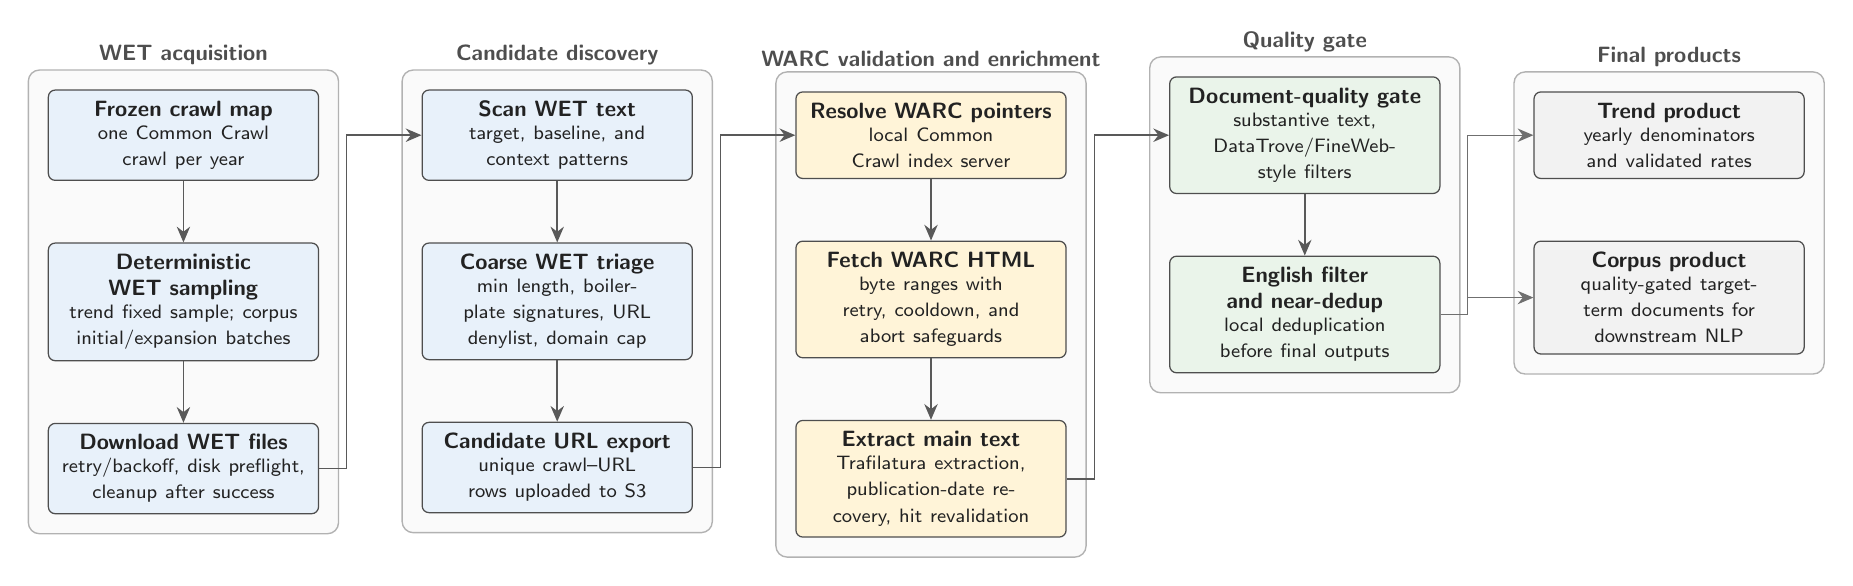
\begin{tikzpicture}[
  font=\sffamily\footnotesize,
  node distance=0.78cm and 0.82cm,
  every node/.style={text=ink}
]

% Column 1: crawl frame and WET acquisition.
\node[wetstage] (crawl) {
  \textbf{Frozen crawl map}\\[-0.15em]
  {\scriptsize one Common Crawl crawl per year}
};
\node[wetstage, below=of crawl] (sample) {
  \textbf{Deterministic WET sampling}\\[-0.15em]
  {\scriptsize trend fixed sample; corpus initial/expansion batches}
};
\node[wetstage, below=of sample] (download) {
  \textbf{Download WET files}\\[-0.15em]
  {\scriptsize retry/backoff, disk preflight, cleanup after success}
};

% Column 2: WET candidate discovery.
\node[wetstage, right=1.30cm of crawl] (scan) {
  \textbf{Scan WET text}\\[-0.15em]
  {\scriptsize target, baseline, and context patterns}
};
\node[wetstage, below=of scan] (triage) {
  \textbf{Coarse WET triage}\\[-0.15em]
  {\scriptsize min length, boilerplate signatures, URL denylist, domain cap}
};
\node[wetstage, below=of triage] (urls) {
  \textbf{Candidate URL export}\\[-0.15em]
  {\scriptsize unique crawl--URL rows uploaded to S3}
};

% Column 3: WARC validation and enrichment.
\node[warcstage, right=1.30cm of scan] (resolve) {
  \textbf{Resolve WARC pointers}\\[-0.15em]
  {\scriptsize local Common Crawl index server}
};
\node[warcstage, below=of resolve] (fetch) {
  \textbf{Fetch WARC HTML}\\[-0.15em]
  {\scriptsize byte ranges with retry, cooldown, and abort safeguards}
};
\node[warcstage, below=of fetch] (extract) {
  \textbf{Extract main text}\\[-0.15em]
  {\scriptsize Trafilatura extraction, publication-date recovery, hit revalidation}
};

% Column 4: quality gate.
\node[qualitystage, right=1.30cm of resolve] (quality) {
  \textbf{Document-quality gate}\\[-0.15em]
  {\scriptsize substantive text, DataTrove/FineWeb-style filters}
};
\node[qualitystage, below=of quality] (langdedup) {
  \textbf{English filter and near-dedup}\\[-0.15em]
  {\scriptsize local deduplication before final outputs}
};

% Column 5: final products.
\node[product, right=1.18cm of quality] (trend) {
  \textbf{Trend product}\\[-0.15em]
  {\scriptsize yearly denominators and validated rates}
};
\node[product, below=of trend] (corpus) {
  \textbf{Corpus product}\\[-0.15em]
  {\scriptsize quality-gated target-term documents for downstream NLP}
};

% Arrows within and across stages.
\draw[flow] (crawl) -- (sample);
\draw[flow] (sample) -- (download);
\draw[flow] (download.east) -- ++(0.35,0) |- (scan.west);

\draw[flow] (scan) -- (triage);
\draw[flow] (triage) -- (urls);
\draw[flow] (urls.east) -- ++(0.35,0) |- (resolve.west);

\draw[flow] (resolve) -- (fetch);
\draw[flow] (fetch) -- (extract);
\draw[flow] (extract.east) -- ++(0.35,0) |- (quality.west);

\draw[flow] (quality) -- (langdedup);
\draw[splitflow] (langdedup.east) -- ++(0.34,0) |- (trend.west);
\draw[splitflow] (langdedup.east) -- ++(0.34,0) |- (corpus.west);

% Stage grouping boxes.
\begin{scope}[on background layer]
  \node[group, fit=(crawl) (sample) (download),
    label={[group label]above:WET acquisition}] {};
  \node[group, fit=(scan) (triage) (urls),
    label={[group label]above:Candidate discovery}] {};
  \node[group, fit=(resolve) (fetch) (extract),
    label={[group label]above:WARC validation and enrichment}] {};
  \node[group, fit=(quality) (langdedup),
    label={[group label]above:Quality gate}] {};
  \node[group, fit=(trend) (corpus),
    label={[group label]above:Final products}] {};
\end{scope}

\end{tikzpicture}
\end{document}
